The Thomas Jefferson National Accelerator Facility, also called Jefferson Lab (JLab), is one of the 17 National Laboratories in the United States \parencite{DepartmentofEnergy2023DepartmentLaboratories}, and functions mainly to deliver high energy, continuous wave (CW) electron beams to fixed-target nuclear and particle physics experiments. The facility was established in 1984 - initially named the Continuous Electron Beam Accelerator Facility (CEBAF) - and first delivered a 4 GeV electron beam on July 1 1994 to one of its three original detector halls. In 2006 efforts began to upgrade the facility to produce an electron beam up to 12 GeV in energy, which was first successfully delivered in 2015, as well as to construct a fourth detector hall for additional physics experiments\parencite{JeffersonLab2023AboutLab}. JLab is also home to a free-electron laser, capable of 10+ kW CW operation \parencite{Benson2007HighAccelerator}. 

\begin{figure}[ht]
    \centering
    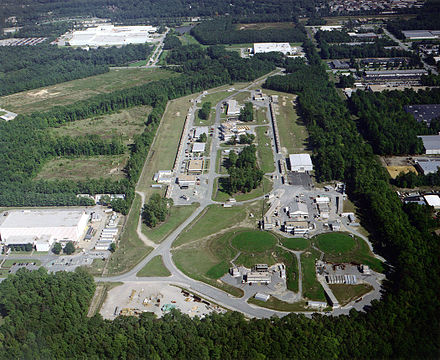
\includegraphics[width=0.8\textwidth]{Chapters/Ch2-Experiment/accel_and_beamline/pics/CEBAF/jlab_wiki.png}
    \caption[Aerial View of JLab]{An aerial view of the Thomas Jefferson National Accelerator Facility \parencite{Wang2010CEBAFOverview}. Note that this picture was taken before the addition of the fourth detector hall (Hall D).}
    \label{fig:jlab_wiki}
\end{figure}

\subsection{Accelerator Facility}
    
    \figref{fig:jlab_accelerator_layout} shows the overarching scheme of the entire accelerator facility relevant for this experiment. Electrons are produced via the photoelectric effect from a 499 MHz pulsed laser impinges on a Gallium Arsenide photocathode \figref{fig:gun}. The CEBAF guns operate at 100 kV and accelerate the electrons through a beam chopper \figref{fig:chopper} to create the desired beam structure \figref{fig:structure} and into the main accelerator circuit, where 1497 MHz superconducting resonator (SRF) cavities provide further acceleration \figref{fig:klystron}. CEBAF's two $\sim$ 1.1 GV linacs accelerate electrons by consist of 50 cryomodules total, with each cryomodule housing 8 7-cell SRF cavities and the liquid helium necessary to cool them, made possible by JLab's 2K liquid helium refrigerator, the largest in the world as of 2023. The electrons are steered around the curved parts of the track by dipole magnets \figref{fig:magnets}, making five complete circulations before delivery to the three western experimental halls, and an additional half circulation to achieve a full 12 GeV beam to Hall D. 
    
    
    \begin{figure}[ht]
        \centering
        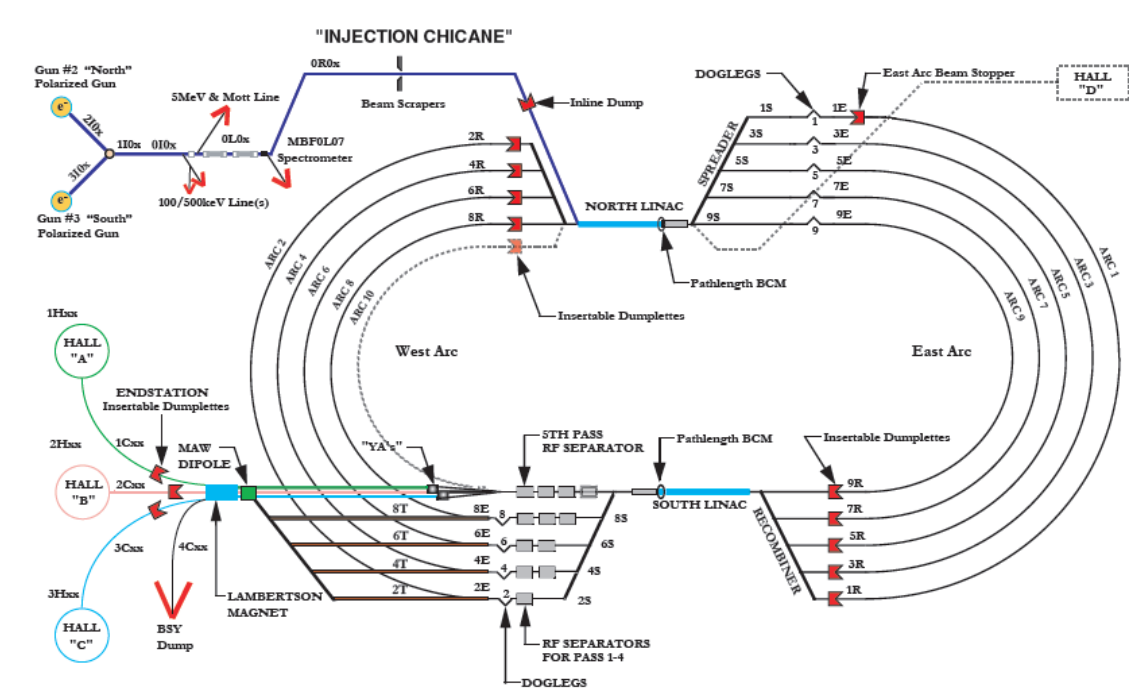
\includegraphics[width=0.8\textwidth]{Chapters/Ch2-Experiment/accel_and_beamline/pics/CEBAF/jlab-accelerator-layout.png}
        \caption[JLab Accelerator Schematic]{Schematic layout of the CEBAF accelerator at JLab. The racetrack configuration has two linear accelerator portions $\sim$ 1/4 mile long, and is $\sim$ 7/8 mile around \parencite{Wang2010CEBAFOverview}.}
        \label{fig:jlab_accelerator_layout}
    \end{figure}
    
    
    \begin{figure}[htb]
        \begin{minipage}[c]{\linewidth}
            \centering
            \subfloat[CEBAF Electron Gun]{\label{fig:gun}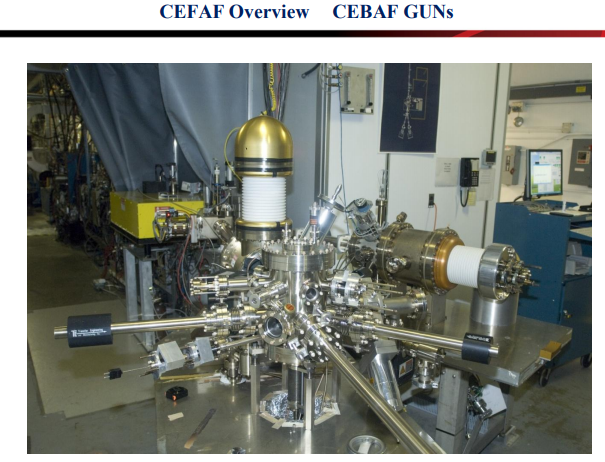
\includegraphics[trim={1 1 1 30},clip,width=0.3\textwidth]{Chapters/Ch2-Experiment/accel_and_beamline/pics/CEBAF/1_CEBAF-guns.png}}
            \subfloat[Beam Chopper]{\label{fig:chopper}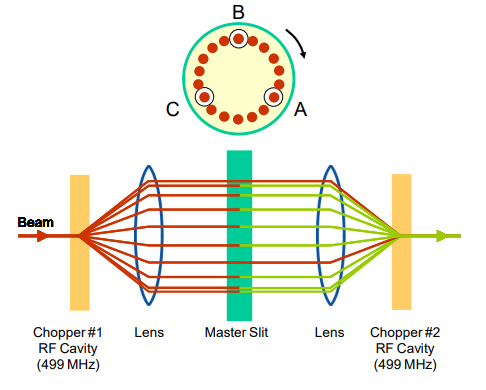
\includegraphics[width=0.3\textwidth]{Chapters/Ch2-Experiment/accel_and_beamline/pics/CEBAF/jlab-chopper.png}}
            \subfloat[CEBAF Beam Structure]{\label{fig:structure}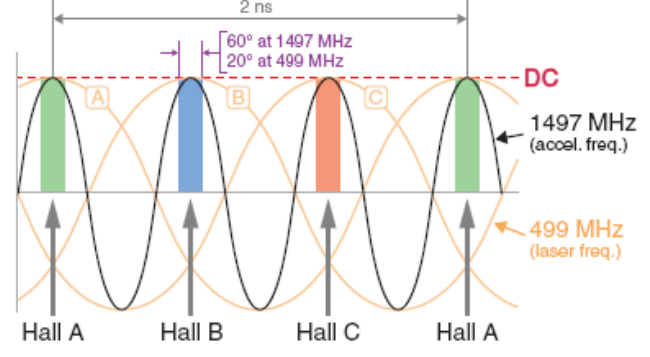
\includegraphics[width=0.3\textwidth]{Chapters/Ch2-Experiment/accel_and_beamline/pics/CEBAF/Jlab-beam-structure.png}}
        \end{minipage}
        \begin{minipage}[c]{\linewidth}
            \centering
            \subfloat[7-cell 1497 MHz Niobium SRF Cavity]{\label{fig:klystron}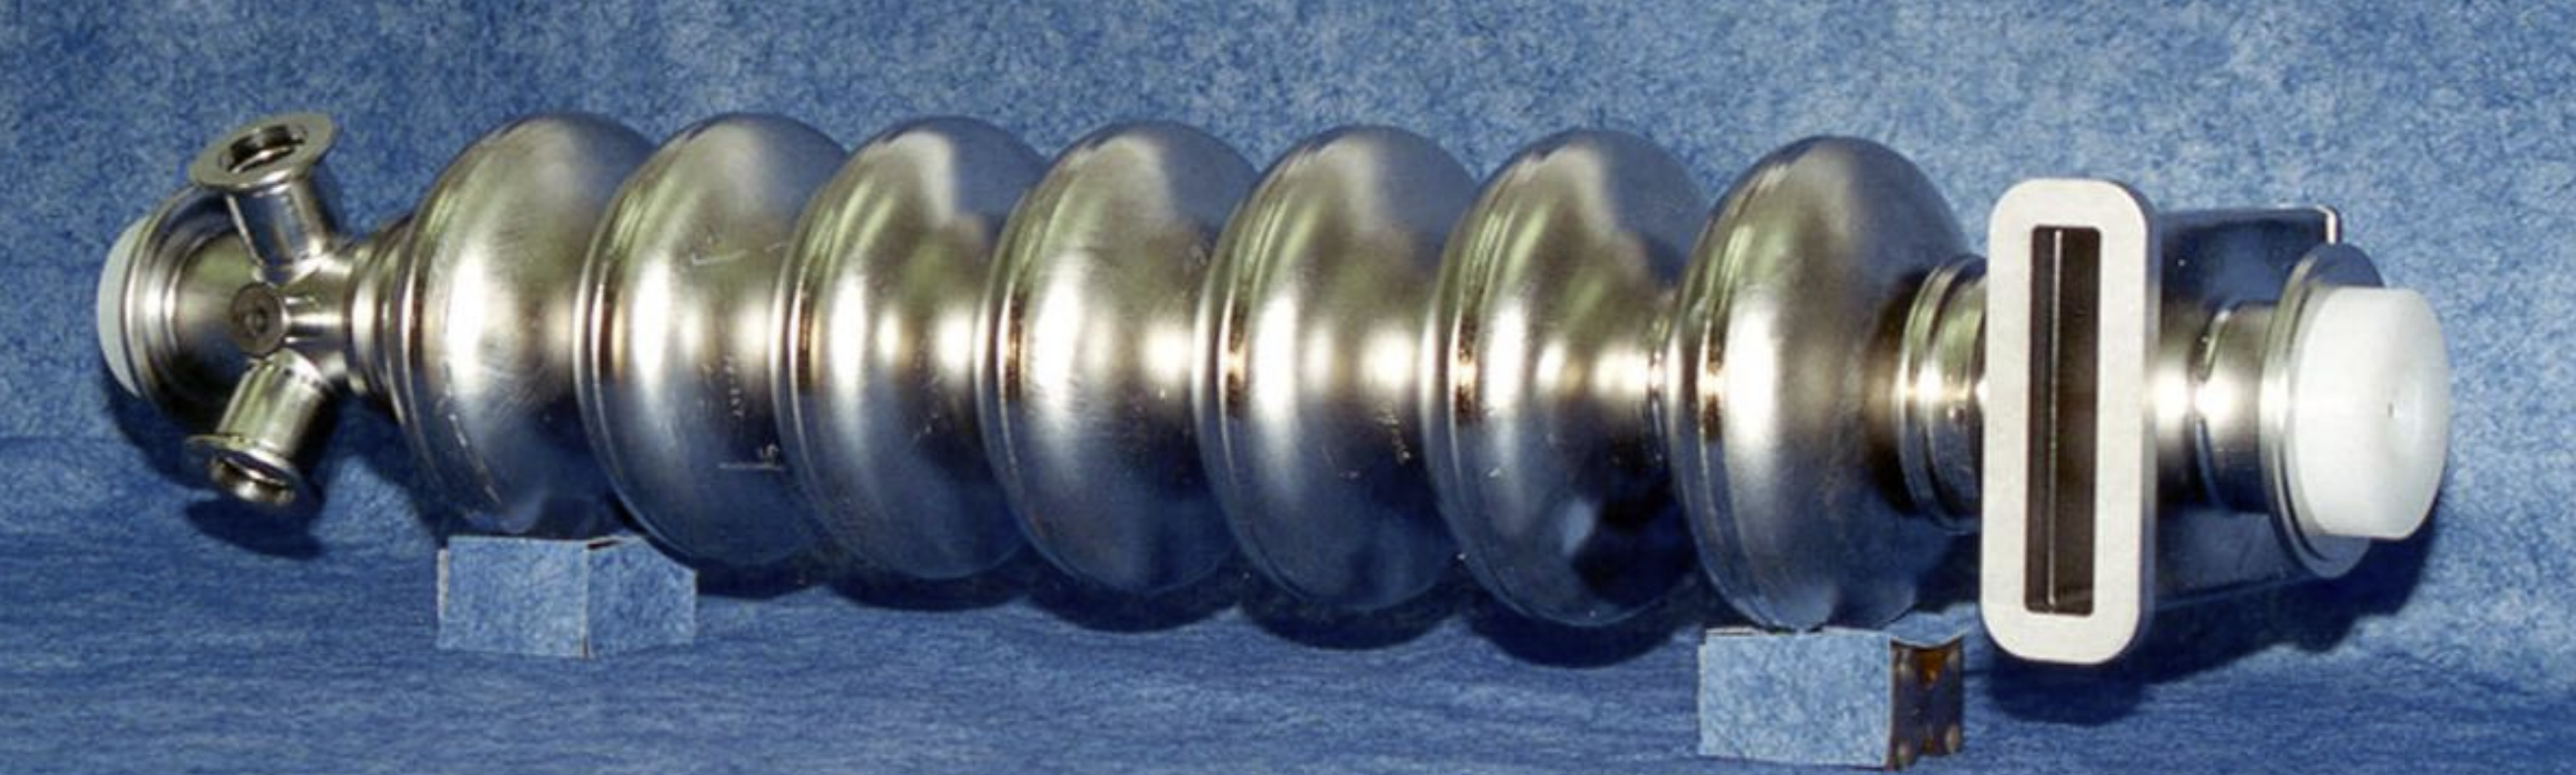
\includegraphics[width=0.4\textwidth]{Chapters/Ch2-Experiment/accel_and_beamline/pics/CEBAF/klystron.png}}
            \hfil
            \subfloat[CEBAF Beamlines]{\label{fig:magnets}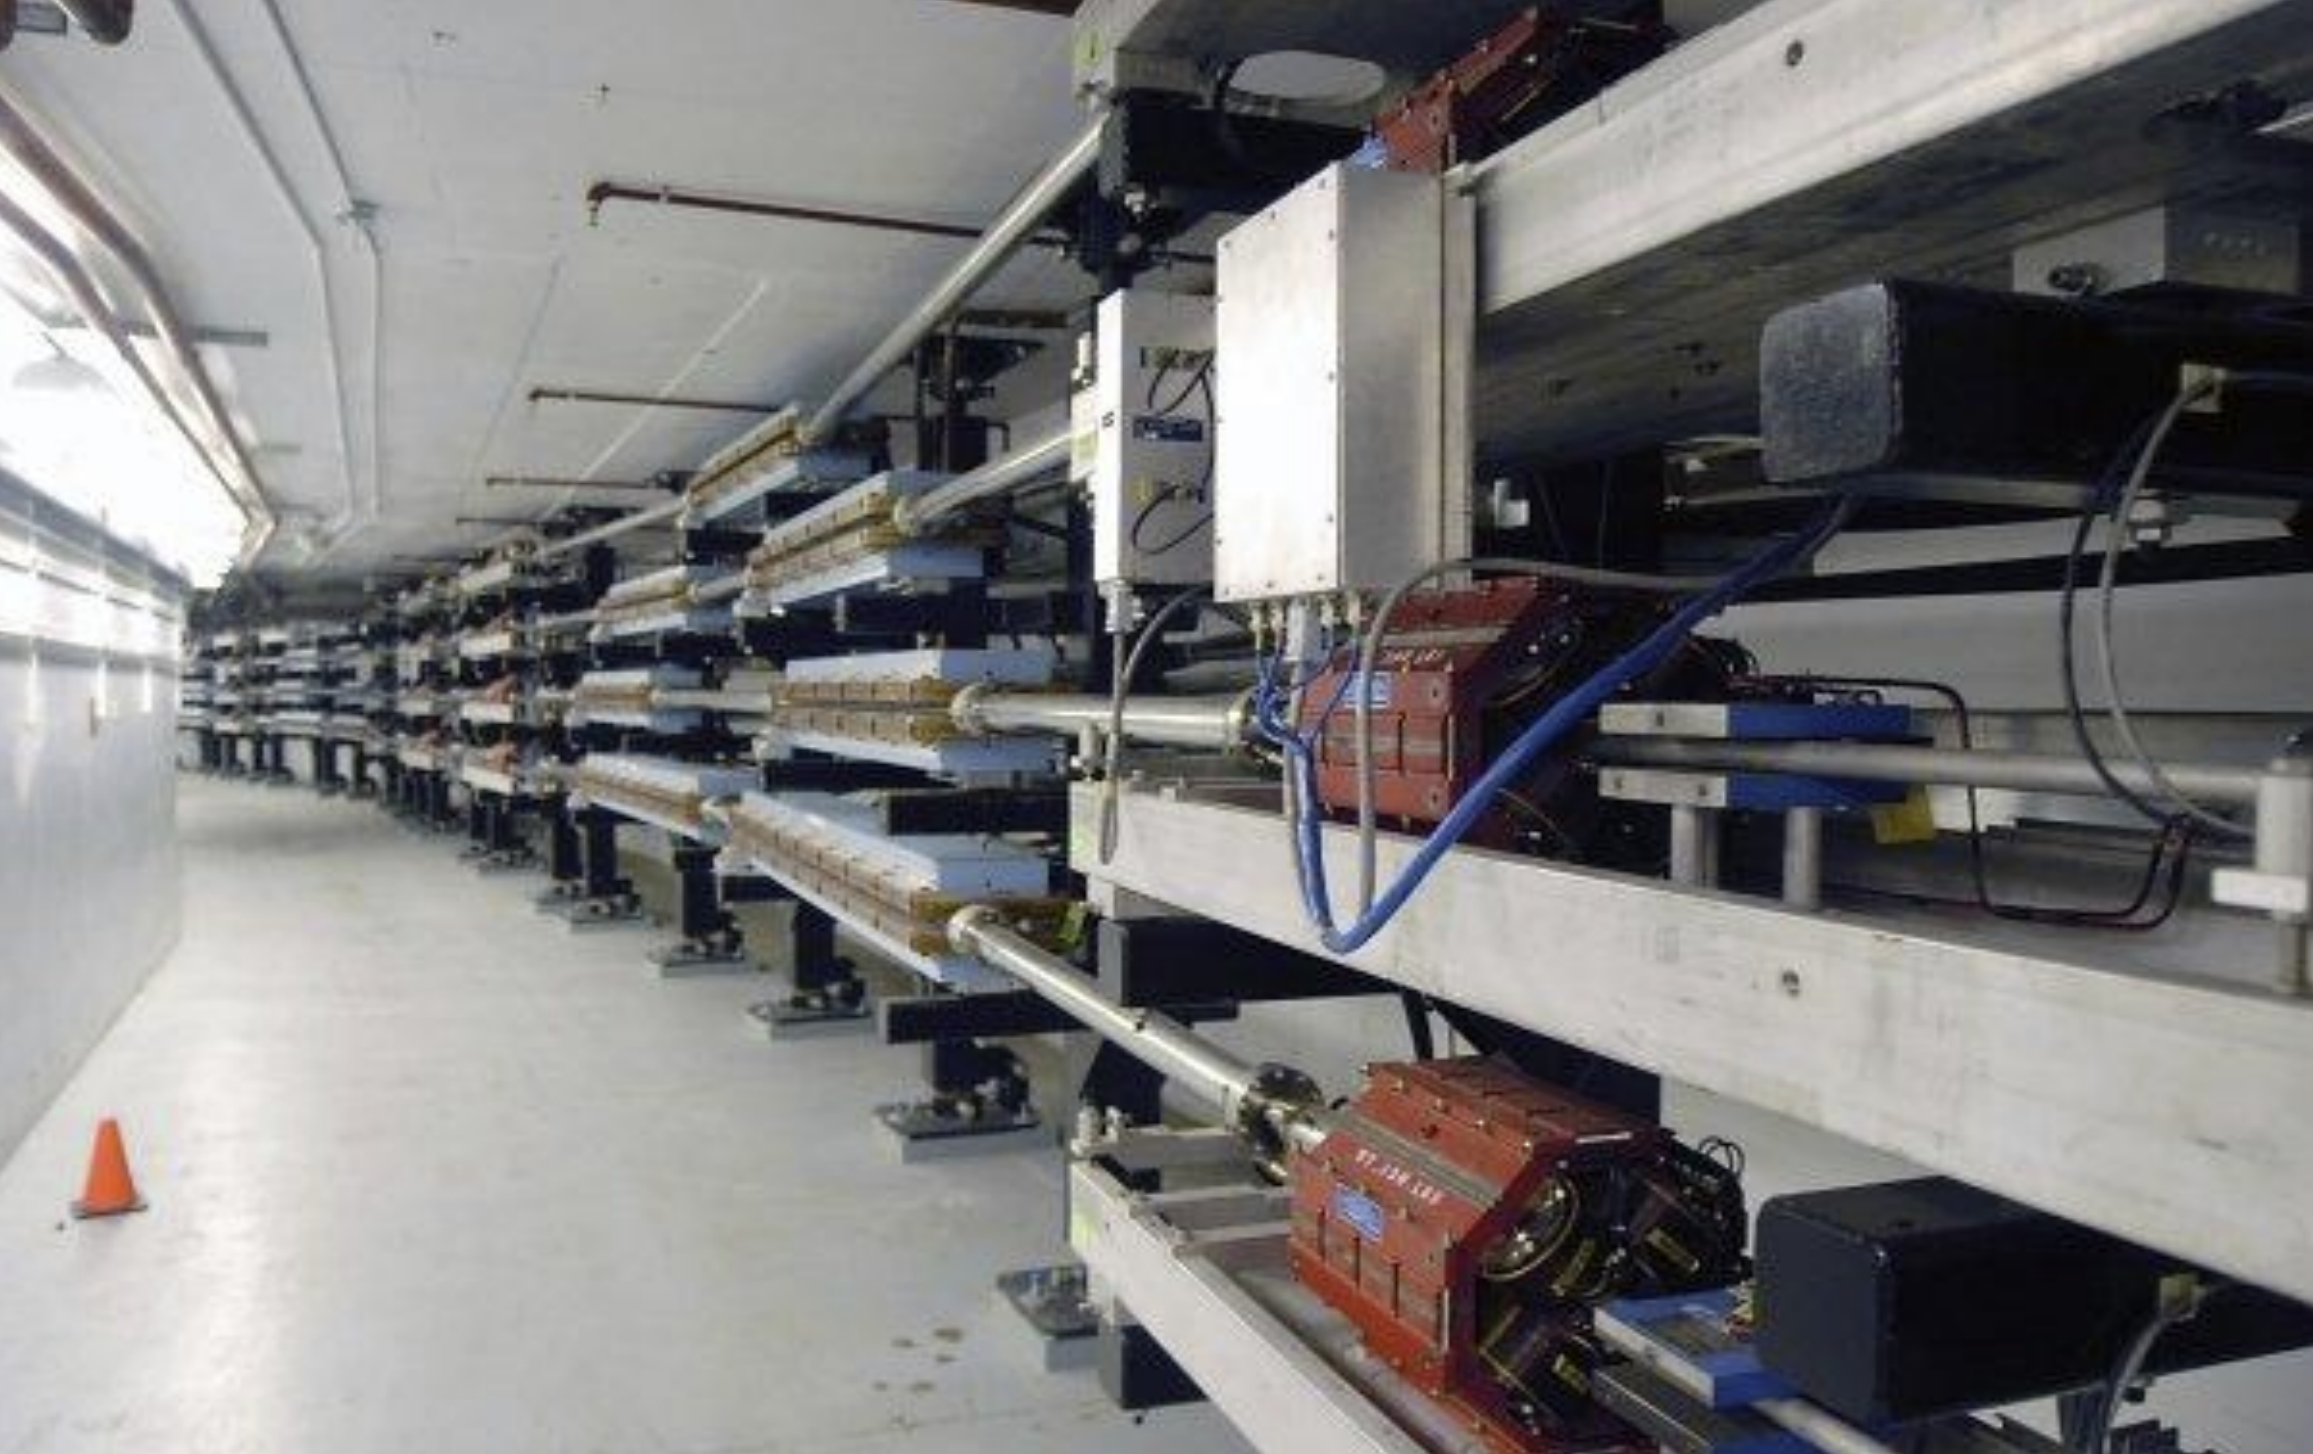
\includegraphics[width=0.4\textwidth]{Chapters/Ch2-Experiment/accel_and_beamline/pics/CEBAF/magnets2.png}}
        \end{minipage}
        \caption[CEBAF Beamline]{Electrons originate from the CEBAF guns (a) and pass through a beam chopper (b) to obtain the desired interlaced beam structure (c). The electrons are accelerated by superconducting RF cavities (d) and steered by dipole magnets (e) to reach an energy of 10.6 GeV before entering detector hall B. Images from \parencite{Wang2010CEBAFOverview}}
        \label{fig:JLab}
    \end{figure}


    \clearpage
    \subsection{Hall B Beamline}

        \begin{table}[h]
                \centering
                \begin{tabular}{rc}
                    Quantity  & Beam Property \\\hline
                    Beam current  & Up to 50 nA \\
                    Beam energy spread  & $10^{-4}$ \\
                    Beam size  & Less than 0.4 mm \\
                    Beam stability  & Less than 0.1 mm \\
                    Beam halo & $10^{-4}$ \\
                    Beam polarization & Up to 85\% \\
                \end{tabular}
            \caption{Beam specifications into Hall B.}
            \label{table:beam-properties}
        \end{table}
        
        The beam enters Hall B with the nominal parameters as specified in Table \ref{table:beam-properties}. Upstream of the target, Hall B uses coincidence double arm \Moller polarimeters \figref{fig:moller} to measure beam polarization within a few percent accuracy. This analysis does not utilize the polarized beam for physics extraction, but it is useful for BSA measurements as well as other physics goals. 
    
            
                \iffalse
                %MORE DETAILS ON MOLLER POLARIMETERY:
                Good for beam energies between 100 MeV and 50 GeV. Polarized beam electrons are scat-
                tered from other polarized electrons in a target, usually magnetized foils. Only a small
                fraction of all the target electrons are polarized, so this method has a small analyzing
                power. Analyzing power is exactly calculable in QED. At high beam energies, analyzing
                power and scattering probability both become independently of beam energy. Maximum
                analyzing power is about 80%, maximum is at 90 degrees scattering angle in C.o.M. Trans-
                versely polarized target can be used to measure transverse beam polarization, but analyzing
                power is only about 10%. 90 degrees C.o.M. translates to a small lab angle with each elec-
                tron at half beam energy, so magnets are used to bend these electrons out to detectors.
                These detectors can be, for example lead glass total absorption cherenkov counters.Since
                the two electrons are corellated, can use things like time coincidence to reduce background,
                although for low duty factor accelerators only one electron is required as statistics would
                otherwise be too low.A main background to this process is Mott scattering with the electron
                radiating off energy after scattering, appearing as a Moller electron
                
                The scattering target is either iron or vanadium permendur (iron-cobalt alloy). Only 2 of
                26 electrons in iron have their spins oriented, leading to a total analyzing power of only 6 percent
                and transverse analyzing power of only 1%. Uncertainties in how magnetized the targets
                actually are corresponds to an uncertainty in analyzing power. There are ’easy’ and ’hard’
                magnetization schemes - easy does a soft magnetization, while hard uses a several tesla mag-
                net to saturate the target. In principle, uncertainties on magnetization in the hard scheme
                can be removed by using the Kerr magneto-optic effect, but this has not ever been imple-
                mented. An important correction is due to the Levchuk effect, where due to momentum
                differences between electrons in different shells, electrons scattered off of polarized electrons
                are more likely to be detected than off of unpolarized electrons. Specifically, inner electrons
                are unpolarized and have a large average momenta, so when struck they can fall outside the
                acceptance of the Moller detectors, while the outer electrons, which are polarized, have a
                small average momentum, and behave as expected. This is up to a 15% effect on polarization
                measurements, and is currently a work in progress.
                \fi

             

            The beam is rasterized onto the target cell \figref{fig:target_cell} is a 5 cm long Kapton cone with 23.66 and 15.08 upstream and downstream diameters respectively, with 30 $\mu$m thick aluminum entrance and exit windows. The target used for this analysis consisted of unpolarized pure liquid hydrogen (LH2) and is located from -5.5 cm (upsteam) to -0.5 cm along the z-axis of the CLAS12 coordinate system \parencite{Baltzell2020ThePerformance}. 
            

            The target is surrounded nearly in 4$\pi$ with detectors as discussed in the next section. The beamline ends in a beam dump and Faraday cup \figref{fig:faraday_cup}, which measures the beam current to allow for absolute cross section determinations. The Faraday cup from the original CLAS experiment and is only rated for 175 Watts (16.5 nA at 10.6 GeV) so a beam blocker is utilized for full-beam runs. More details can be found in found in \parencite{Mecking2003TheCLAS} %link to own fraday cup paper \cite{Johnston2019RealizationElectrons}
            
  
    
    \begin{figure}[ht]
        \centering
        % First row with 3 columns
        \begin{minipage}[b]{0.3\linewidth}
            \subfloat[Upstream (top) and downstream (bottom) view of \Moller polarimeters \parencite{Joo2002ElectronPolarimeter}.]{\label{fig:moller}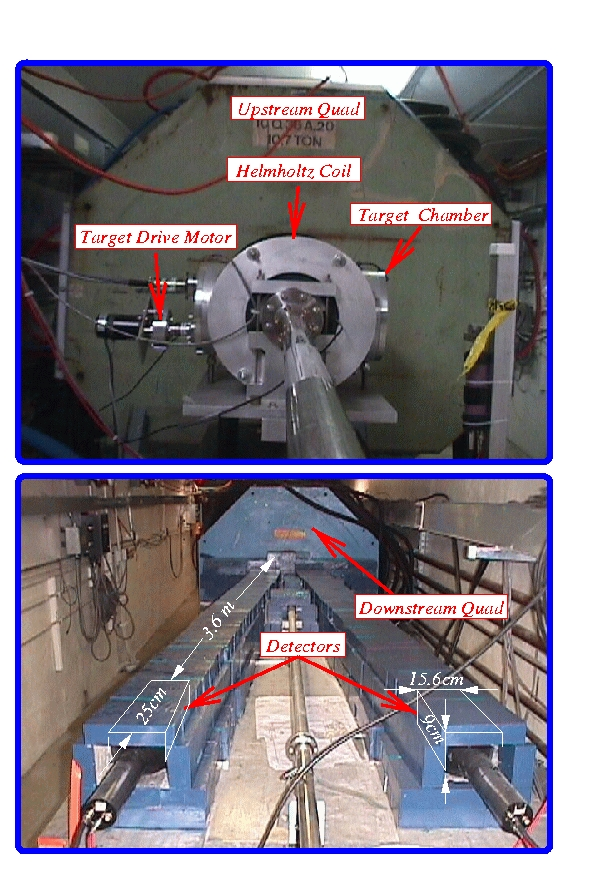
\includegraphics[width=\linewidth]{Chapters/Ch2-Experiment/accel_and_beamline/pics/hallB/hall-b-poll-2.jpg}}
        \end{minipage}
        \hfill
        \begin{minipage}[b]{0.3\linewidth}
            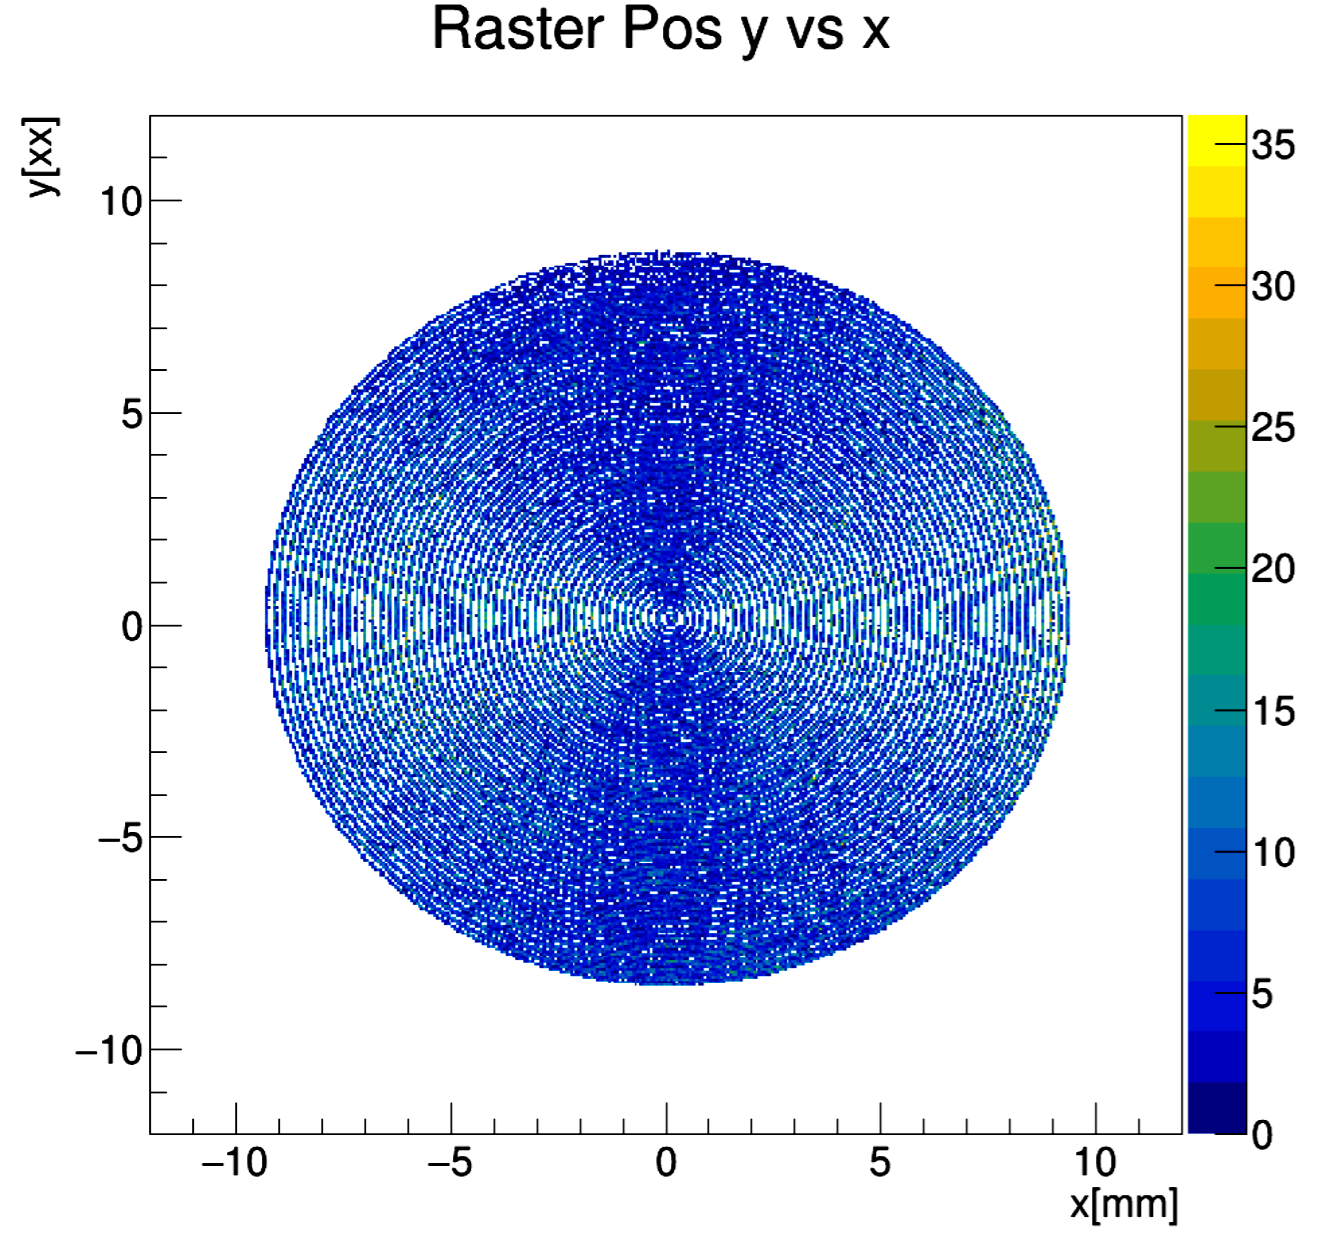
\includegraphics[width=.8\linewidth]{Chapters/Ch2-Experiment/accel_and_beamline/pics/hallB/beam_rastering_new.png}
            \vfill
            \subfloat[Raserterization pattern (top) on CLAS12 target (bottom) \parencite{Achenbach2022HallReport}.]{\label{fig:target_cell}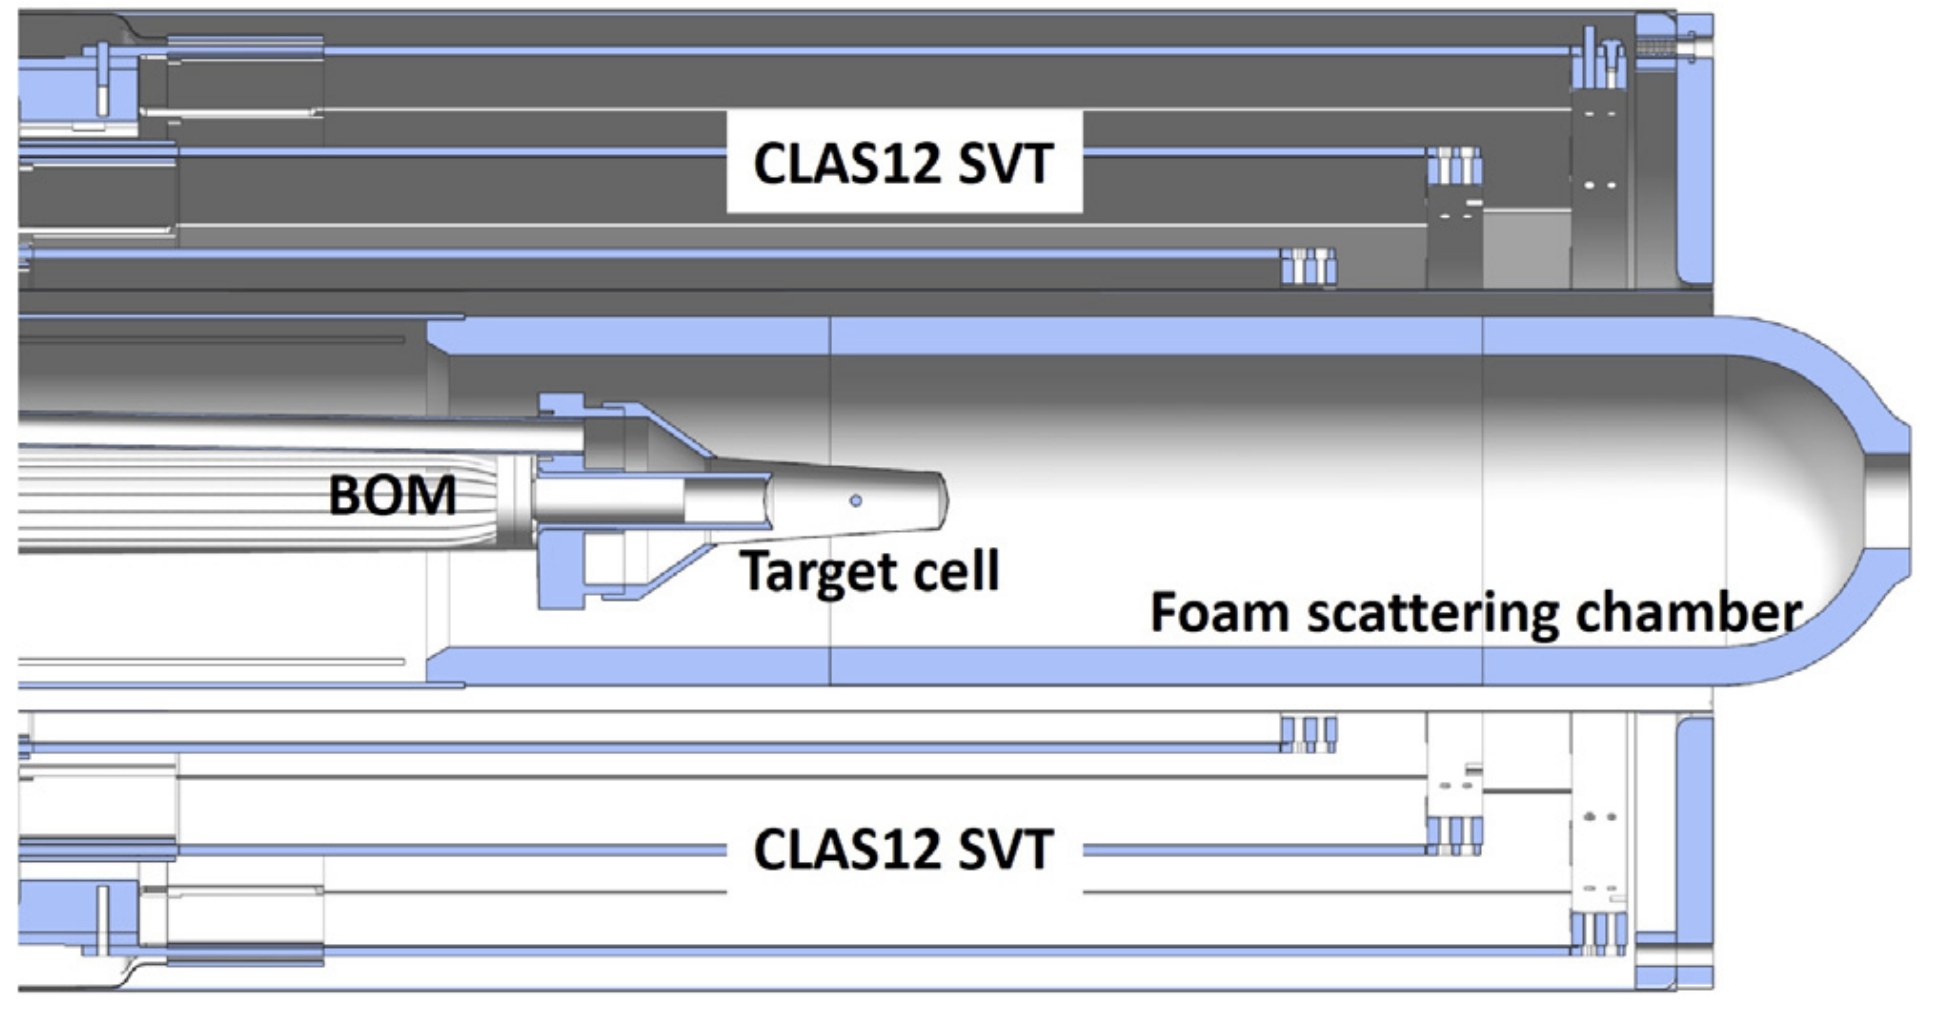
\includegraphics[width=\linewidth]{Chapters/Ch2-Experiment/accel_and_beamline/pics/hallB/target.png}}
        \end{minipage}
        \hfill
        \begin{minipage}[b]{0.3\linewidth}
            \subfloat[Faraday cup, shown removed from operating position \parencite{Achenbach2022HallReport}.]{\label{fig:faraday_cup}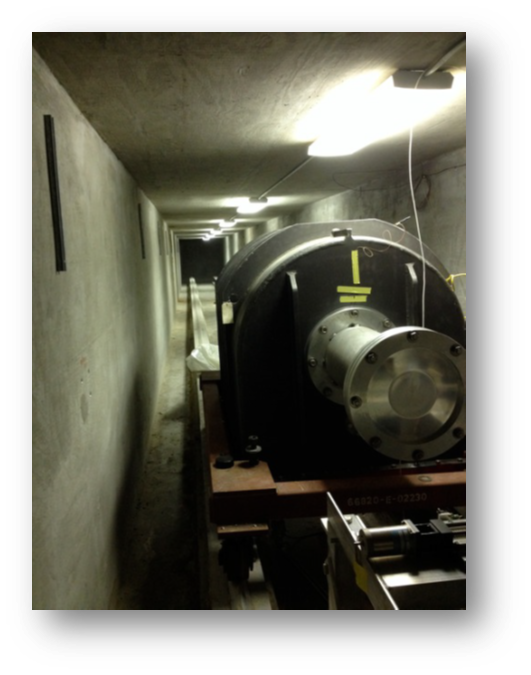
\includegraphics[trim={2.5cm 1cm 1cm 2cm},clip,width=\linewidth]{Chapters/Ch2-Experiment/accel_and_beamline/pics/hallB/beamdump1.png}}
        \end{minipage}
        % Second row with 1 column
        \begin{minipage}[b]{\linewidth}
            \centering
            \subfloat[Hall B beamline, from \parencite{Baltzell2020ThePerformance}.]{\label{fig:beamline}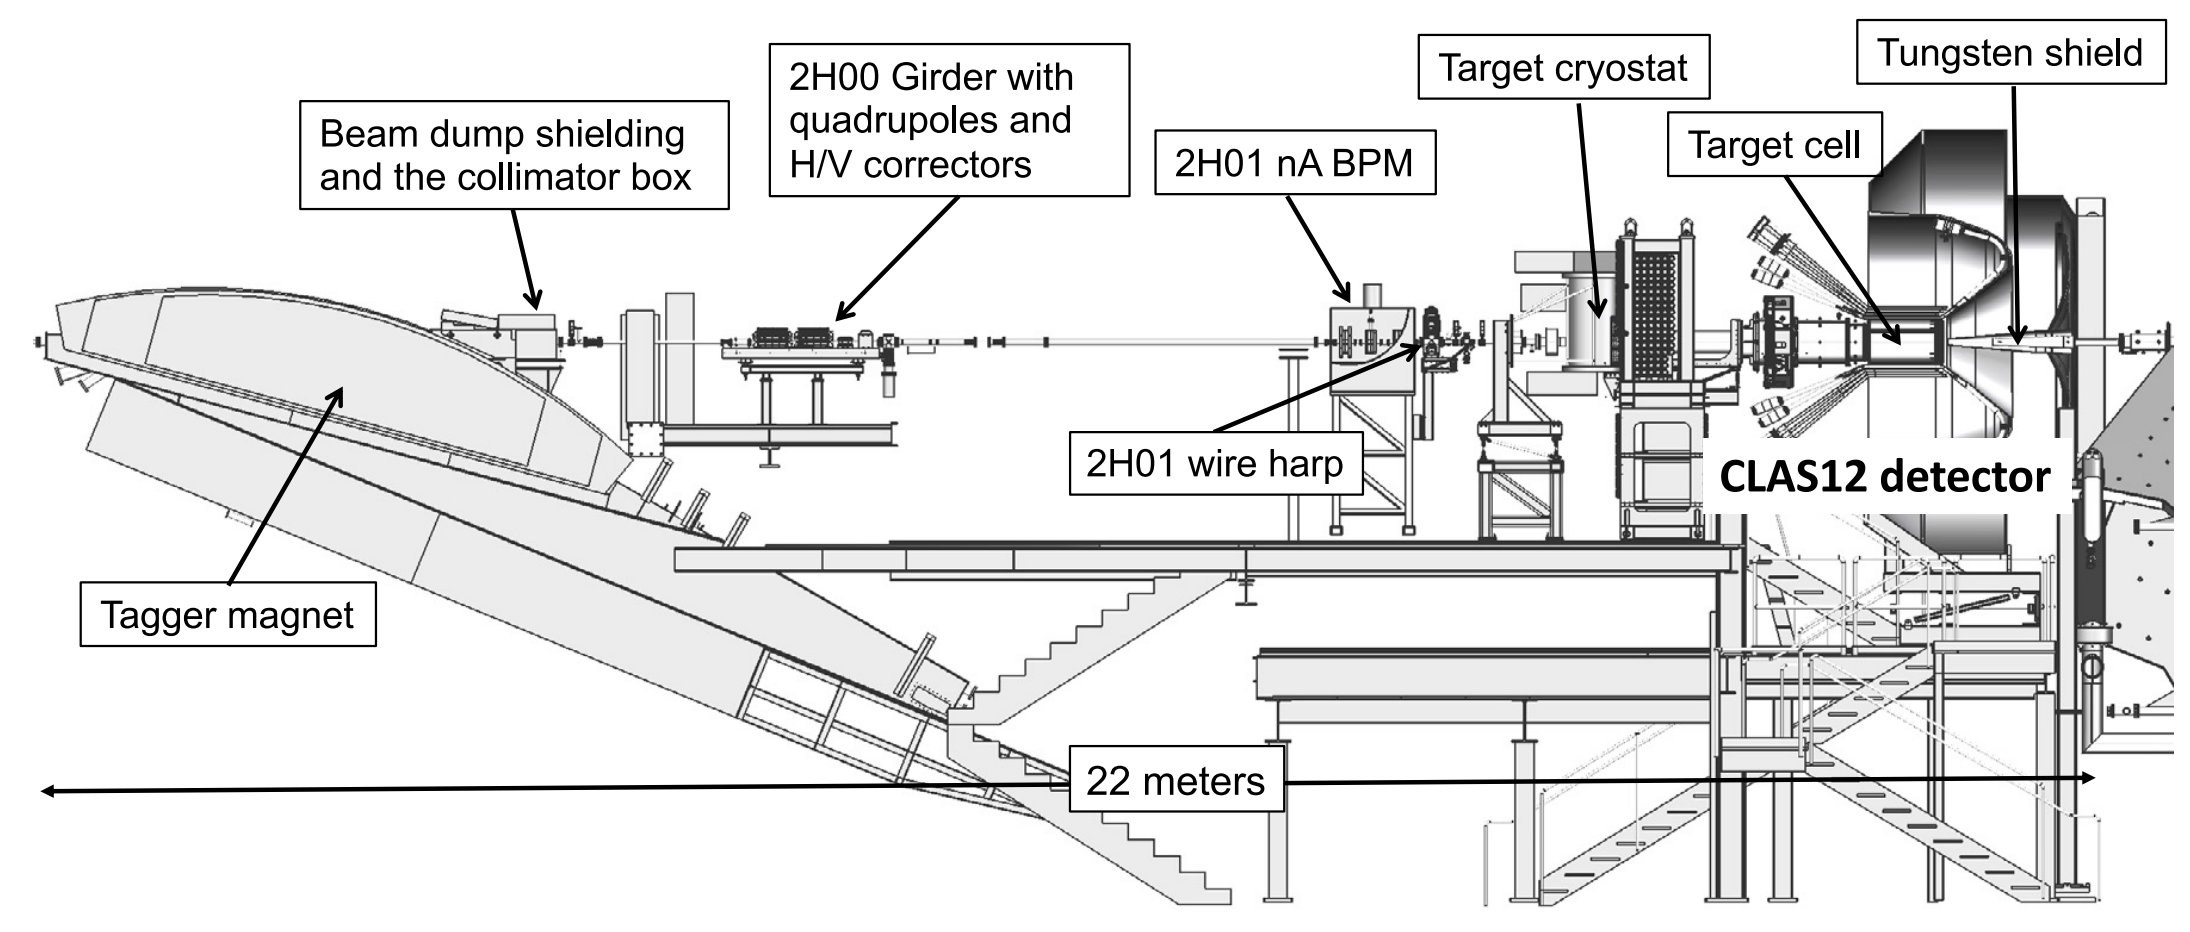
\includegraphics[width=0.9\linewidth]{Chapters/Ch2-Experiment/accel_and_beamline/pics/hallB/beamline.png}}
        \end{minipage}
        \caption[Hall B Beamline]{Overview of Hall B beamline. After \Moller polarimeters (a), the electron beam is rasterized on CLAS12 target (b) with interactions recorded by the CLAS12 detector while the rest of the beam ends at the beam dump and Faraday cup (c). (d) shows the scaled detector hall layout, with the \Moller polarimeters being located to the left of the Tagger magnet and the Faraday cup to the right of the CLAS12 detector package.}
        \label{fig:allfigures}
    \end{figure}

    \clearpage
